% CVPR 2024 camera-ready layout for the course report.
\documentclass[10pt,twocolumn,letterpaper]{article}
\usepackage[pagenumbers]{cvpr}
% Use the template's Times font shapes when compiling with XeTeX.
\ifdefined\XeTeXversion
    \usepackage[T1]{fontenc}
\fi
\usepackage{amsmath,amssymb,booktabs,graphicx}
\usepackage[table]{xcolor}
\definecolor{cvprblue}{rgb}{0.21,0.49,0.74}
\definecolor{neighborhighlight}{RGB}{226,239,250}
\usepackage[pdfusetitle,breaklinks,colorlinks,allcolors=cvprblue]{hyperref}

\title{Semantic Neighbor Reassignment for Collision Resolution\texorpdfstring{\\}{ }in Generative Recommendation}
\author{M1YAN\\
Deep Learning Methods and Applications\\
Course Project}

\newcommand{\codebooks}{\ensuremath{256/256/256/64}}
\newcommand{\RankingRows}{%
Sequential & 0.00974 / \textbf{1.581\%} & 0.01319 / \underline{2.656\%} & 0.01740 / 4.314\% & \underline{0.01674} / \textbf{2.892\%} & \underline{0.02183} / \textbf{4.478\%} & \textbf{0.02998} / \textbf{7.711\%} \\%
Global popularity & \underline{0.01003} / 1.560\% & 0.01333 / 2.579\% & \underline{0.01775} / 4.349\% & 0.01518 / 2.301\% & 0.02062 / 3.980\% & 0.02771 / 6.872\% \\%
Fixed-prefix ZCR & 0.00969 / 1.567\% & \underline{0.01338} / \textbf{2.712\%} & 0.01762 / 4.399\% & 0.01299 / 2.332\% & 0.01822 / 3.949\% & 0.02535 / 6.810\% \\%
Zero-weight control & 0.00969 / 1.567\% & \underline{0.01338} / \textbf{2.712\%} & 0.01762 / 4.399\% & 0.01299 / 2.332\% & 0.01822 / 3.949\% & 0.02535 / 6.810\% \\%
Neighbors (0.25, 3) & 0.00985 / \underline{1.574\%} & 0.01326 / 2.649\% & 0.01767 / \underline{4.406\%} & 0.01670 / 2.736\% & 0.02181 / \underline{4.353\%} & \underline{0.02931} / \underline{7.369\%} \\%
Neighbors (0.50, 3) & 0.00978 / \textbf{1.581\%} & 0.01311 / 2.621\% & \textbf{0.01785} / \textbf{4.497\%} & 0.01486 / 2.301\% & 0.01951 / 3.762\% & 0.02705 / 6.779\% \\%
\rowcolor{neighborhighlight} Neighbors (1.00, 3) & \textbf{0.01009} / \underline{1.574\%} & \textbf{0.01340} / 2.614\% & 0.01759 / 4.286\% & \textbf{0.01823} / \underline{2.767\%} & \textbf{0.02218} / 4.011\% & 0.02875 / 6.685\% \\%
Neighbors (0.50, 1) & 0.00976 / 1.553\% & 0.01291 / 2.530\% & 0.01697 / 4.153\% & 0.01426 / 2.488\% & 0.01895 / 3.949\% & 0.02649 / 6.996\% \\%
}

\newcommand{\SweepRows}{%
$(0.25, 3)$ & 0.028049 & \underline{0.021811} \\%
$(0.50, 3)$ & \underline{0.028052} & 0.019512 \\%
\rowcolor{neighborhighlight} $(1.00, 3)$ & 0.027767 & \textbf{0.022175} \\%
$(0.50, 1)$ & \textbf{0.028149} & 0.018949 \\%
}


\begin{document}
\maketitle

\begin{abstract}
Generative recommenders predict a discrete identifier for the next item.
When several items share a three-code prefix, the fourth code must distinguish them.
We study a fourth-code assignment that preserves text-based relationships within a prefix.
Starting from fixed-prefix Zero-Collision Reassignment (ZCR), we optimize residual distortion together with a graph-weighted distance between the fourth-code centroids assigned to semantic neighbors.
We compare eight settings on Amazon Beauty using a fixed \codebooks{} codebook and a 20,000-update training budget.
The highest test mean for collided targets is 0.02218 NDCG@10 at neighbor weight $\lambda=1.0$ and $k=3$, a 21.7\% relative increase over ZCR with gains in all three paired seeds.
For groups of three to four items, it scores 0.03253 versus 0.02696 for sequential assignment.
Sequential assignment leads collided-target Hit@10 and both collided-target metrics at rank 20.
The subgroup and cutoff results identify where semantic reassignment improves ranking.
\end{abstract}

\section{Introduction}
\label{sec:intro}
A semantic identifier (SID) represents an item as a short sequence of discrete codes.
TIGER established a generative retrieval pipeline in which an encoder--decoder Transformer predicts the next item's code sequence from past interactions~\cite{rajput2023generative}.
Residual quantization groups related items into shared prefixes.
A collision group needs distinct final codes so the decoder can identify its members.

The last-code assignment also defines what the recommender must learn.
A minimum-distortion assignment chooses a fourth-level centroid that fits each item's residual while satisfying uniqueness.
We ask whether the same assignment can also preserve relationships between items that share a prefix.
For example, two shades of the same lipstick should receive distinct identifiers.
Their textual similarity provides a reason to place their assigned centroids nearby.

Our contribution is a prefix-local graph objective added to fixed-prefix ZCR.
We compare it with sequential numbering, global popularity, and minimum-distortion assignment under shared tokenization and training conditions.
We analyze ranking across cutoffs, prefix-group sizes, training frequencies, and user activity.
\Cref{fig:pipeline} shows where the assignment policy enters the pipeline.

\begin{figure*}[t]
    \centering
    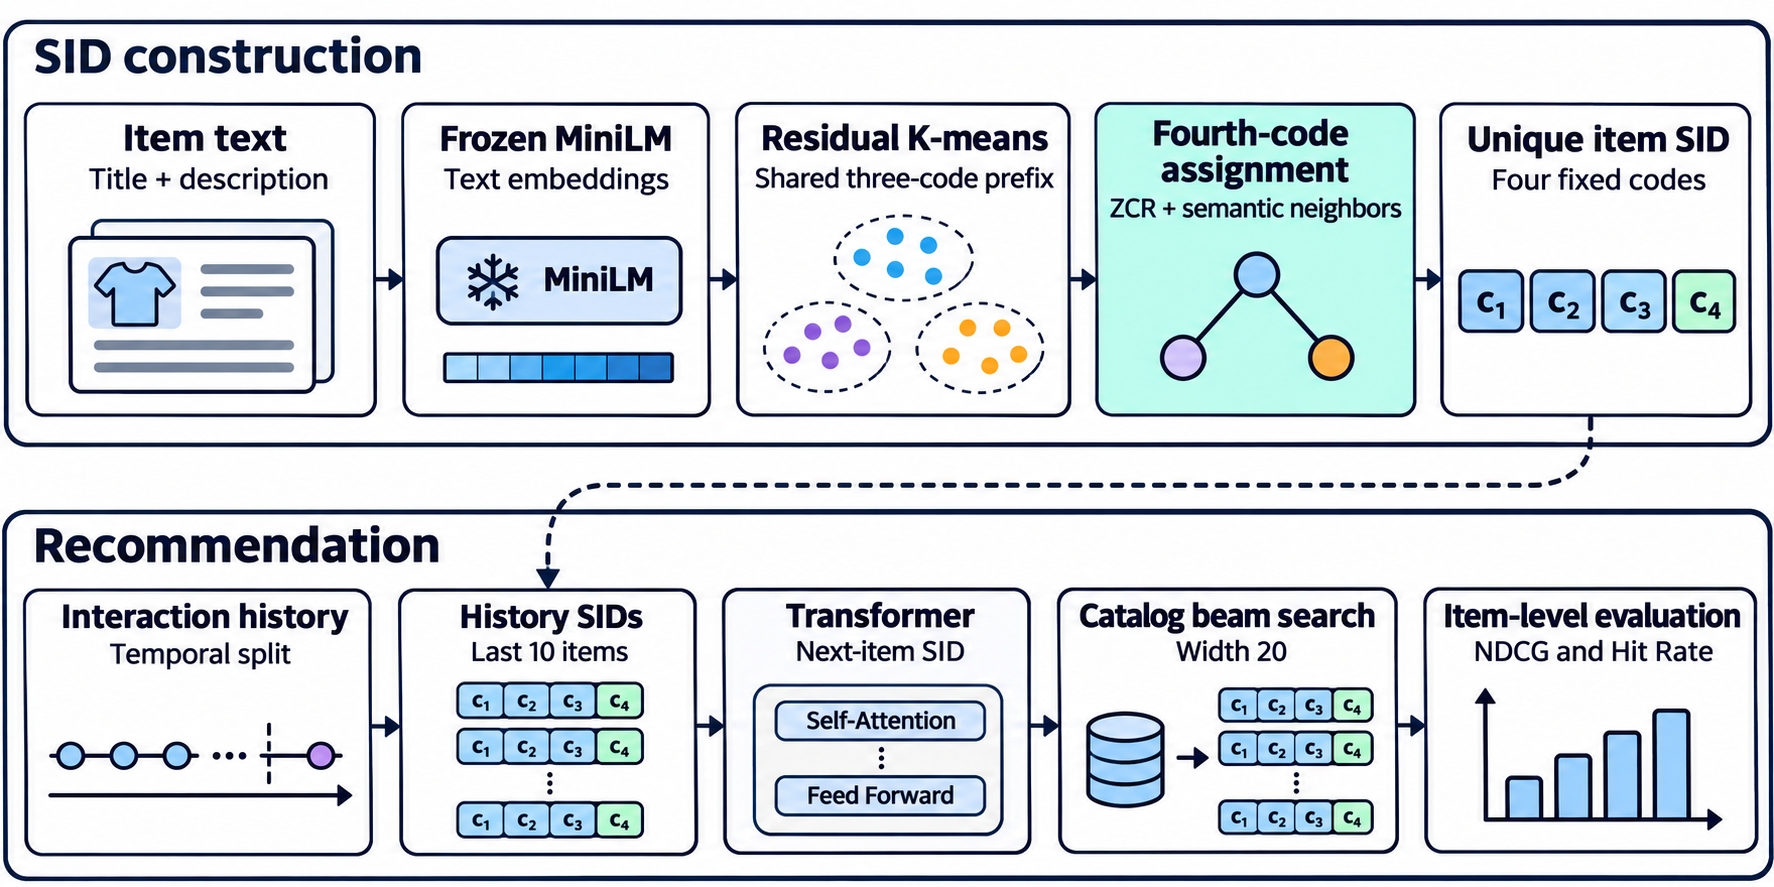
\includegraphics[width=\textwidth]{figures/pipeline-imagegen.png}
    \caption{End-to-end pipeline. Every policy uses the same text embeddings, prefix assignments, fourth-code capacity, interaction split, generator, and decoding configuration. Fourth-code assignment determines the SID mapping used for training and retrieval.}
    \label{fig:pipeline}
\end{figure*}

\section{Related Work}

\paragraph{Sequential recommendation and generative retrieval.}
Self-attentive sequential models such as SASRec summarize a user's interaction history and score catalog items using learned item embeddings~\cite{kang2018sasrec}.
In generative retrieval, the model predicts a sequence of tokens that identifies an item.
TIGER quantizes item content embeddings into a hierarchy of semantic codes and trains a sequence-to-sequence Transformer to predict the next item's identifier~\cite{rajput2023generative}.
This design lets multiple items share coarse codes, so the generator can learn a broad category and then refine the prediction at later positions.
The underlying residual quantization idea also appears in RQ-VAE, which represents an input with successive codewords that approximate its remaining residual~\cite{lee2022residual}.

\paragraph{Learning semantic identifiers.}
Work on item tokenization studies which signals the identifier should preserve.
LC-Rec learns collaborative item indices and uses alignment tasks to connect the indices to a language model~\cite{zheng2024lcrec}.
LETTER combines hierarchical quantization, collaborative alignment, and a diversity objective for code assignments~\cite{wang2024letter}.
Adaptive Silhouette Trees allocate branching factors according to the local item distribution, allowing different prefixes to have different numbers of child nodes~\cite{hadad2026branches}.
These methods show how collaborative signals and codebook design can shape identifiers.
Our experiment fixes the prefix tree and varies how existing fourth-code centroids are assigned within each group.

\paragraph{Collision resolution and item-level evaluation.}
TIGER appends ordinal suffixes to make identifiers unique when quantized prefixes collide~\cite{rajput2023generative}.
Volodkevich et al.\ study suffix policies that carry content, popularity, or collaborative signals while keeping the quantizer, generator, and code length fixed~\cite{volodkevich2026last}.
Zhang et al.\ show that a shared complete SID can inflate SID-level metrics when a match leaves the underlying item ambiguous.
Their collision-corrected evaluation scores at the item level, and ZCR uses minimum-cost reassignment to make identifiers unique~\cite{zhang2026faithful}.
We use fixed-prefix ZCR as a comparison and as the starting point for graph-based reassignment.
The added objective preserves relationships between text neighbors, and we measure how its gains vary with prefix-group size and ranking cutoff.

\section{Prefix-Local Semantic Reassignment}
\label{sec:method}

\subsection{Text embeddings and codebooks}
We concatenate each training-catalog item's title and description, tokenize up to 128 tokens, and use frozen \texttt{all-MiniLM-L6-v2}~\cite{minilm}.
Masked mean pooling and $\ell_2$ normalization produce a 384-dimensional unit vector $x_i$.
Seven catalog entries with missing text receive a shared fallback string.

Residual K-means fits the levels sequentially.
Each of the first three levels assigns the nearest centroid and subtracts it before the next level.
Let $p_i$ be the resulting three-code prefix and $r_i$ the remaining residual.
A fourth K-means fit to those residuals provides 64 available centroids $c_1,\dots,c_{64}$.
All policies share these centroids and the three-code prefixes.
For a prefix group $G$ of $m$ items, we assign distinct fourth codes $a_i$ within $G$.
Different prefixes can reuse the same code, and each complete SID identifies exactly one item.

\subsection{Fixed-prefix ZCR}
\label{sec:zcr}
Let $D_i(a)=\|r_i-c_a\|_2^2$.
Fixed-prefix ZCR solves the rectangular linear assignment problem
\begin{equation}
    a^{\mathrm{ZCR}} =
        \operatorname*{arg\,min}_{a\ \mathrm{injective}}
        \sum_{i\in G} D_i(a_i).
    \label{eq:zcr}
\end{equation}
The solution accounts for competition for the same code across the entire group.
We use SciPy's linear sum assignment implementation.
All resulting SIDs are fixed before recommender training.

\subsection{Graph-weighted objective}
\label{sec:graph}
Item $i$ selects up to $k$ other members of $G$ by cosine similarity $x_i^{\mathsf T} x_j$.
An undirected edge is included when either item selects the other.
Its weight $w_{ij}$ is the positive part of the cosine similarity.
The assignment objective is
\begin{align}
    J(a) &= \frac{1}{m}\sum_{i\in G} D_i(a_i) + \lambda P(a), \label{eq:objective}\\
    P(a) &=
        \frac{\sum_{i<j} w_{ij}\,\|c_{a_i}-c_{a_j}\|_2^2}
             {\sum_{i<j} w_{ij}}. \label{eq:pair}
\end{align}
Here $P(a)=0$ for a group without positive edges.
The first term measures mean item distortion.
The second measures weighted pairwise distortion, so semantically closer items exert a stronger pull on the assignment of their respective centroids.
The distance depends on centroid vectors.
The code indices act as categorical labels.

Starting from \cref{eq:zcr}, the search makes at most four sweeps over a group.
For each item, assigning an empty code changes one item, and assigning an occupied code swaps the two items' codes.
We evaluate the full change in \cref{eq:objective}, including affected graph edges, and execute the candidate that yields the largest strict decrease.
A sweep with zero accepted moves terminates the search.
Both move types preserve uniqueness.

\paragraph{Illustrative swap.}
Suppose A--B and B--C have edge weights 0.8 and 0.6, respectively.
Swapping A's and B's codes preserves their mutual centroid distance.
If B--C squared distance drops from 0.09 to 0.04, the graph term decreases by $0.6(0.09-0.04)/1.4=0.02143$.
An increase of 0.01667 in mean residual distortion still gives a decrease of 0.00476 in $J$ at $\lambda=1$, so the swap is accepted.

\section{Experimental Protocol}
\label{sec:protocol}

\subsection{Data and time split}
We use Amazon Reviews 2014 Beauty ratings and metadata~\cite{mcauley2015image}.
We retain the earliest event per user--item pair and apply iterative user and item 5-core filtering.
The result contains 22,363 users, 12,101 items, and 198,502 interactions.
The global $90$th timestamp percentile defines the test boundary.
The $90$th percentile among events at or before that boundary defines the validation boundary.
Boundary timestamps belong to the earlier partition.

Users with at least two pre-validation interactions provide training examples.
Their interactions define the training catalog and item frequencies.
For each eligible validation or test user, we select the last target within the corresponding time window.
A retained example has a target in the training catalog and at least one earlier catalog item in its visible history.
\Cref{tab:data} summarizes the samples.
The catalog contains 958 collided prefixes, with a maximum group size of 20.
All policies produce 11,805 unique complete SIDs.

\begin{table}[t]
    \centering
    \small
    \begin{tabular}{lrrr}
        \toprule
        Population & Total & Collided & Share \\
        \midrule
        Catalog items     & 11,805  & 2,329  & 19.73\% \\
        Train examples    & 140,086 & 29,856 & 21.31\% \\
        Validation targets & 5,662  & 1,306  & 23.07\% \\
        Test targets       & 4,744  & 1,072  & 22.60\% \\
        \bottomrule
    \end{tabular}
    \caption{Dataset sizes. A collided item shares its three-code prefix with at least one other catalog item.}
    \label{tab:data}
\end{table}

\subsection{Baselines and comparison settings}
\label{sec:baselines}
The comparison changes only the policy used to assign the fourth code within each prefix.
All settings use the same catalog, three-code prefixes, 64 fourth-code centroids, interaction splits, training budget, and decoding configuration.

\begin{itemize}
    \item \textbf{Sequential.} Sort the items within each prefix by catalog item ID (ASIN order), then assign codes $0,1,\dots,m-1$.
    This implements the ordinal disambiguation policy used in TIGER~\cite{rajput2023generative}.
    \item \textbf{Global popularity.} Rank catalog items by training interaction count and map each rank to one of 64 equal-rank bins.
    Process items within each prefix in descending frequency order and assign the closest available code to each item's preferred bin.
    \item \textbf{Fixed-prefix ZCR.} Use the one-to-one minimum-distortion matching in \cref{eq:zcr}.
    Each edge cost is the squared distance from an item's third-level residual to a candidate fourth-level centroid~\cite{zhang2026faithful}.
    \item \textbf{Zero-weight control.} Use the neighbor assignment implementation with $\lambda=0$.
    Its catalog mapping is identical to fixed-prefix ZCR, providing a check on the effect of the graph term.
    \item \textbf{Semantic neighbors.} Initialize with ZCR and apply the objective in \cref{eq:objective}.
    The reference setting is $(\lambda,k)=(0.50,3)$.
    The sensitivity analysis adds $(0.25,3)$ and $(1.00,3)$ to vary the graph weight and $(0.50,1)$ to vary the number of neighbors.
\end{itemize}

\subsection{Generator and checkpoint selection}
We use a 687,232-parameter Transformer with two encoder and two decoder layers, model width 96, four attention heads, feed-forward width 384, and dropout 0.1.
Its input is the SID sequence for up to ten recent items.
Teacher forcing supervises the four output positions using equal-weight cross-entropy.
AdamW uses a learning rate of 0.001, batch size 64, weight decay 0.01, and gradient clipping at 1.0.

Each policy uses seeds 17, 42, and 73 and matches both initialization and batch order by seed.
The training budget is 20,000 updates, with validation every 500 updates.
For each seed we select the checkpoint with the highest collided-target validation NDCG@10.
Full-set NDCG@10 and then the earliest checkpoint break ties.
The median selected step across 24 runs is 18,000.
\Cref{fig:training} shows curves from the same training trajectories.
On a single NVIDIA A800 80 GB, the median training time is 247.8 seconds per run and median full validation decode time is 0.80 seconds.
Peak allocated CUDA memory is 168.7 MiB per run.

\begin{figure*}[t]
    \centering
    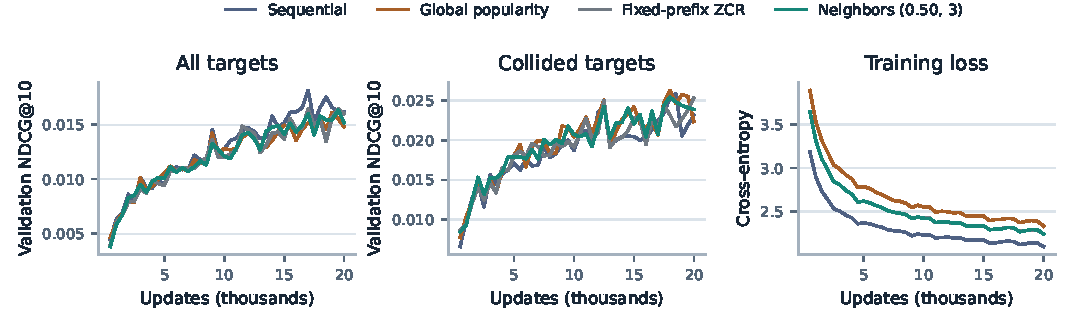
\includegraphics[width=\textwidth]{figures/training_curves.pdf}
    \caption{Mean validation NDCG@10 and training cross-entropy from the original 20,000-update runs. The zero-weight control follows ZCR exactly. Test scores use each seed's validation-selected checkpoint.}
    \label{fig:training}
\end{figure*}

\subsection{Item-level evaluation}
A catalog trie restricts beam search to valid SIDs, with beam width 20.
Each complete SID maps to one item.
For one held-out target at rank $r\le K$, Hit@$K$ is 1 and NDCG@$K$ is $1/\log_2(r+1)$.
A target outside the top $K$ receives zero on both metrics.
We average across test examples and then across seeds.
The primary cutoff is 10, with additional evaluation at 5 and 20.
Collided subsets are further grouped by prefix size, target training frequency, and a user's number of pre-validation interactions in the filtered dataset.

\section{Ranking Results}
\label{sec:results}

\begin{table*}[t]
    \centering
    \small
    \setlength{\tabcolsep}{4pt}
    \resizebox{\textwidth}{!}{%
        \begin{tabular}{lrrrrrr}
            \toprule
            Fourth-code policy
            & \multicolumn{3}{c}{All test targets ($n=4{,}744$)}
            & \multicolumn{3}{c}{Collided targets ($n=1{,}072$)} \\
            \cmidrule(lr){2-4}\cmidrule(lr){5-7}
            Neighbors $(\lambda,k)$ & @5 & @10 & @20 & @5 & @10 & @20 \\
            \midrule
            \RankingRows
            \bottomrule
        \end{tabular}%
    }
    \caption{Test ranking under a fixed 20,000-update budget. Each cell reports NDCG / Hit Rate, averaged across three seeds. \textbf{Bold} and \underline{underline} indicate the best and second-best values, respectively, for each metric within each cutoff and target group. Ties share the same marking.}
    \label{tab:ranking}
\end{table*}

\subsection{Comparison with fixed-prefix ZCR}
At $(\lambda,k)=(1.00,3)$, collided NDCG@10 increases from 0.01822 to 0.02218.
The absolute difference is 0.00396, a 21.7\% relative increase.
The three paired-seed differences are $+0.00355$, $+0.00302$, and $+0.00531$.
Hit@10 rises from 3.949\% to 4.011\% on the same targets.

The mean and sample standard deviation of collided NDCG@10 are $0.02218\pm0.00317$ for $(1.00,3)$ and $0.01822\pm0.00401$ for ZCR.
The sample standard deviation of the paired differences is 0.00120.
The original neighbor setting $(0.50,3)$ gains 0.00130 on average over ZCR and wins one of three paired comparisons.
At $\lambda=0$, the assignment and all reported scores match ZCR for all three seeds.

\subsection{Comparison with sequential and popularity}
\Cref{tab:ranking} shows that $(1.00,3)$ also leads collided NDCG@5.
At @10, its collided NDCG exceeds global popularity by 0.00155 and sequential by 0.00034.
It beats sequential in one of the three paired seeds (\cref{fig:paired}).
Sequential assignment leads collided Hit@5, Hit@10, and both collided @20 metrics.

On the full test set, $(1.00,3)$ leads NDCG@5 and NDCG@10.
The full-set NDCG@10 difference relative to ZCR is 0.00002.
ZCR and its zero-weight control lead full-set Hit@10, and the original neighbor setting leads both full-set @20 metrics.
NDCG rewards earlier matches, while Hit credits every match within the cutoff equally.
The strongest graph-assignment gains appear in the early ranks for collided targets.

\begin{figure*}[t]
    \centering
    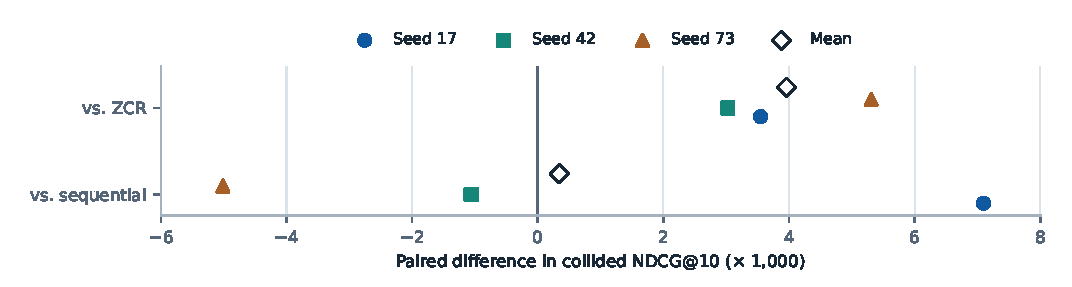
\includegraphics[width=.85\textwidth]{figures/paired_seeds.pdf}
    \caption{Paired differences in collided NDCG@10 for neighbors $(1.00,3)$ against fixed-prefix ZCR and sequential assignment. Each point compares runs with the same seed. Diamonds show mean paired differences.}
    \label{fig:paired}
\end{figure*}

\section{Where Semantic Reassignment Helps}
\label{sec:cohorts}

\begin{figure*}[t]
    \centering
    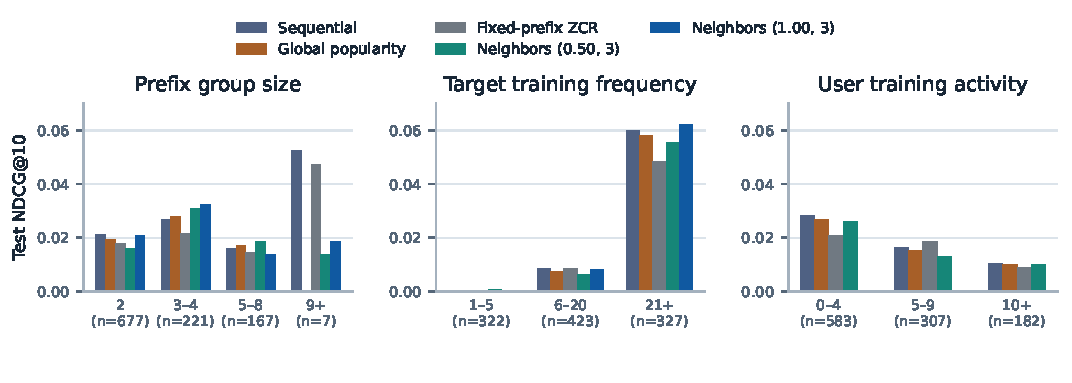
\includegraphics[width=\textwidth]{figures/cohorts.pdf}
    \caption{Collided-target NDCG@10 by prefix-group size, target training frequency, and user training activity. The activity panel uses the original policy set and the reference neighbor configuration. Parenthesized counts are test targets per seed.}
    \label{fig:cohorts}
\end{figure*}

\paragraph{Prefix-group size.}
For groups of three to four items, $(1.00,3)$ scores 0.03253 and $(0.50,3)$ scores 0.03101, ahead of global popularity (0.02794), sequential assignment (0.02696), and ZCR (0.02168).
Both neighbor settings outperform sequential in all three paired seeds.
With at least three group members, a swap can preserve the edge between two items while changing their distances to a third, as illustrated in \cref{sec:graph}.

Pairs account for 677 of 1,072 collided targets.
For these pairs, $(1.00,3)$ improves over ZCR in all three seeds, from 0.01767 to 0.02090 in the mean.
Sequential scores 0.02131.
A swap in a two-item group preserves its only edge distance, whereas moving to an empty code can change it.
For groups of five to eight items, $(0.50,3)$ reaches 0.01851 against 0.01690 for global popularity.
Groups of nine or more contain seven test targets.

\paragraph{Target training frequency.}
Among collided targets with at least 21 training interactions, $(1.00,3)$ reaches 0.06235, compared with 0.04859 for ZCR and 0.06020 for sequential.
It exceeds ZCR in all three seeds.
In the 6--20 interaction bin, sequential reaches 0.00856 compared with 0.00800 for $(1.00,3)$.
In the 1--5 interaction bin, all plotted means are below 0.001.
\Cref{fig:cohorts} shows that the largest absolute gain over ZCR appears among more frequently observed targets.

\paragraph{User training activity.}
For collided targets from users with 0--4 training-period interactions, the original neighbor setting reaches 0.02600 against ZCR's 0.02082, with improvements in all three seeds.
Sequential reaches 0.02841 in this band.
ZCR leads among users with 5--9 interactions.
For users with at least 10 interactions, the four plotted means span 0.00899--0.01036.
Target frequency and user activity capture different sources of training supervision.

\section{Parameter Sensitivity}
\label{sec:sweep}

\begin{figure*}[t]
    \centering
    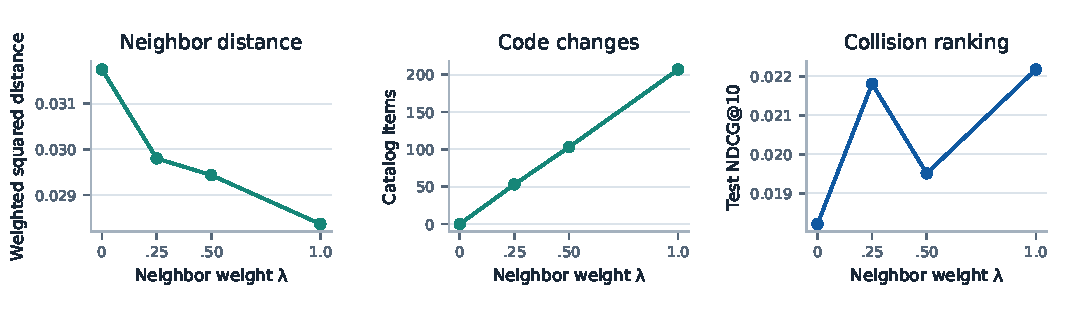
\includegraphics[width=\textwidth]{figures/weight_sweep.pdf}
    \caption{Effect of $\lambda$ at $k=3$. Centroid distance is measured on the same reference graph for every setting. Code changes count catalog items whose final code differs from fixed-prefix ZCR.}
    \label{fig:sweep}
\end{figure*}

\subsection{Assignment geometry}
At $k=3$, increasing $\lambda$ from 0 to 1 reduces the weighted centroid distance from 0.03175 to 0.02837 on a common reference graph, a 10.7\% decrease.
Catalog-wide mean residual distortion moves from 0.32090 to 0.32099.
Weights 0.25, 0.50, and 1.00 change 53, 103, and 207 catalog codes, respectively.
The weight 1.00 changes the fourth code of 66 test targets.
The geometry changes consistently as the weight increases, while the test ranking curve peaks at $\lambda=1.0$ after a dip at $\lambda=0.5$ (\cref{fig:sweep}).
The Transformer learns token embeddings and classification heads from interactions, so centroid proximity enters the generation task through the labels.

\subsection{Reference, validation-selected, and top test settings}
\begin{table}[t]
    \centering
    \small
    \begin{tabular}{lrr}
        \toprule
        Neighbors $(\lambda,k)$ & Validation & Test \\
        \midrule
        \SweepRows
        \bottomrule
    \end{tabular}
    \caption{Collided-target NDCG@10 for the positive-weight sweep. Validation scores use each seed's selected checkpoint. \textbf{Bold} and \underline{underline} mark the best and second-best means in each column.}
    \label{tab:sweep}
\end{table}
The original $(0.50,3)$ setting serves as the reference for the ablation.
The validation selection rule chooses $(0.50,1)$ among the four positive-weight neighbors.
Among all policies, global popularity leads the validation mean at 0.02830.
The highest test mean belongs to $(1.00,3)$.
\Cref{tab:sweep} shows these distinct roles and keeps the original default visible.

The design varies $\lambda$ from 0 to 1 at $k=3$ and compares $k=1$ and $k=3$ at $\lambda=0.50$.
It estimates sensitivity along both axes.
A full interaction comparison would also pair $k=1$ with $\lambda=0.25$ and $\lambda=1.00$.
A validation-selected default for a new evaluation can then be confirmed on an independent temporal split or category.

\section{Conclusion}
Prefix-local semantic reassignment adds item-pair structure to collision resolution while preserving unique SIDs.
On Beauty at fixed code length and training budget, the weight 1.00 setting improves collided NDCG@10 over fixed-prefix ZCR in all three seeds.
Both strong neighbor settings outperform sequential numbering in groups of three to four items across all seeds.
Sequential numbering leads collided Hit@10 and the collided @20 metrics.
The choice of fourth-code policy therefore changes early ranking and retrieval coverage in different ways.

\bibliographystyle{ieeenat_fullname}
\bibliography{references}
\end{document}
